% This example is meant to be compiled with lualatex or xelatex
% The theme itself also supports pdflatex
\PassOptionsToPackage{unicode}{hyperref}
\documentclass[aspectratio=1610, 10pt]{beamer}

% Load packages you need here
\usepackage{polyglossia}
\setmainlanguage{german}

\usepackage{csquotes}

\usepackage{tikz-feynman}
\usepackage{tikz}
\usepackage{siunitx}
\usepackage{braket}

\usepackage{amsmath}
\usepackage{amssymb}
\usepackage{mathtools}

\usepackage{hyperref}
\usepackage{bookmark}
\usepackage{chronosys}
\usepackage{setspace}

\usepackage[]{biblatex}
\usepackage{filecontents}
\begin{filecontents}{literatur2.bib}
	@article{Hadjiivanov:2018lgp,
    author         = "Hadjiivanov, Ludmil",
    title          = "{Neutrino, parity violaton, V-A: a historical survey}",
    year           = "2018",
    eprint         = "1812.11629",
    archivePrefix  = "arXiv",
    primaryClass   = "physics.hist-ph",
    SLACcitation   = "%%CITATION = ARXIV:1812.11629;%%"
	}
	@article{PhysRev.105.1681.2,
	  title = {Nuclear Emulsion Evidence for Parity Nonconservation in the Decay Chain ${\ensuremath{\pi}}^{+}\ensuremath{-}{\ensuremath{\mu}}^{+}\ensuremath{-}{e}^{+}$},
	  author = {Friedman, J. I. and Telegdi, V. L.},
	  journal = {Phys. Rev.},
	  volume = {105},
	  issue = {5},
	  pages = {1681--1682},
	  numpages = {0},
	  year = {1957},
	  month = {Mar},
	  publisher = {American Physical Society},
	  doi = {10.1103/PhysRev.105.1681.2}
	}
	@article{GORTER1948504,
		title = "A new suggestion for aligning certain atomic nucleï",
		journal = "Physica",
		volume = "14",
		number = "8",
		pages = "504",
		year = "1948",
		issn = "0031-8914",
		doi = "https://doi.org/10.1016/0031-8914(48)90004-4",
		author = "C.J Gorter"
	}
	@article{PhysRev.75.213,
	  title = {On the Production of Nuclear Polarization},
	  author = {Rose, M. E.},
	  journal = {Phys. Rev.},
	  volume = {75},
	  issue = {1},
	  pages = {213--213},
	  numpages = {0},
	  year = {1949},
	  month = {01},
	  publisher = {American Physical Society},
	  doi = {10.1103/PhysRev.75.213}
	}
	@article{PhysRev.104.254,
	  title = {Question of Parity Conservation in Weak Interactions},
	  author = {Lee, T. D. and Yang, C. N.},
	  journal = {Phys. Rev.},
	  volume = {104},
	  issue = {1},
	  pages = {254--258},
	  numpages = {0},
	  year = {1956},
	  month = {10},
	  publisher = {American Physical Society},
	  doi = {10.1103/PhysRev.104.254}
	}
	@article{PhysRev.105.1413,
	  title = {Experimental Test of Parity Conservation in Beta Decay},
	  author = {Wu, C. S. and Ambler, E. and Hayward, R. W. and Hoppes, D. D. and Hudson, R. P.},
	  journal = {Phys. Rev.},
	  volume = {105},
	  issue = {4},
	  pages = {1413--1415},
	  numpages = {0},
	  year = {1957},
	  month = {02},
	  publisher = {American Physical Society},
	  doi = {10.1103/PhysRev.105.1413}
	}
	@article{PhysRev.105.1415,
	  title = {Observations of the Failure of Conservation of Parity and Charge Conjugation in Meson Decays: the Magnetic Moment of the Free Muon},
	  author = {Garwin, Richard L. and Lederman, Leon M. and Weinrich, Marcel},
	  journal = {Phys. Rev.},
	  volume = {105},
	  issue = {4},
	  pages = {1415--1417},
	  numpages = {0},
	  year = {1957},
	  month = {02},
	  publisher = {American Physical Society},
	  doi = {10.1103/PhysRev.105.1415}
	}
	@article{doi:10.1080/14786440208520296,
		author = { E.   Ambler  and  M.A.   Grace  and  H.   Halban  and  N.   Kurti  and  H.   Durand  and  C.E.   Johnson  and  H.R.   Lemmer },
		title = {Nuclear polarization of cobalt 60},
		journal = {The London, Edinburgh, and Dublin Philosophical Magazine and Journal of Science},
		volume = {44},
		number = {349},
		pages = {216-218},
		year  = {1953},
		publisher = {Taylor & Francis},
		doi = {10.1080/14786440208520296}
	}
	@article {Cox544,
		author = {Cox, R. T. and McIlwraith, C. G. and Kurrelmeyer, B.},
		title = {Apparent Evidence of Polarization in a Beam of β-Rays},
		volume = {14},
		number = {7},
		pages = {544--549},
		year = {1928},
		doi = {10.1073/pnas.14.7.544},
		publisher = {National Academy of Sciences},
		issn = {0027-8424},
		journal = {Proceedings of the National Academy of Sciences}
	}
	@article{PhysRev.106.340,
	  title = {Remarks on Possible Noninvariance under Time Reversal and Charge Conjugation},
	  author = {Lee, T. D. and Oehme, Reinhard and Yang, C. N.},
	  journal = {Phys. Rev.},
	  volume = {106},
	  issue = {2},
	  pages = {340--345},
	  numpages = {0},
	  year = {1957},
	  month = {04},
	  publisher = {American Physical Society},
	  doi = {10.1103/PhysRev.106.340}
	}
	@article{doi:10.1080/14786441008520365,
		author = { R.H.   Dalitz },
		title = {CXII. On the analysis of τ-meson data and the nature of the τ-meson},
		journal = {The London, Edinburgh, and Dublin Philosophical Magazine and Journal of Science},
		volume = {44},
		number = {357},
		pages = {1068-1080},
		year  = {1953},
		publisher = {Taylor & Francis},
		doi = {10.1080/14786441008520365}
	}
	@article{Chase,
		author = { C.T. Chase },
		title = {The scattering of fast electrons by metals. II. Polarization by double scattering at right angles},
		journal = {Phys. Rev. Lett.},
		volume = {36},
		pages = {1060-1065},
		year  = {1930}
	}
	@online{nobelprize,
	  author = {Magdolna Hargittai},
	  title = {Credit where credit’s due?},
	  url = {https://physicsworld.com/a/credit-where-credits-due/},
	  urldate = {2019-10-22}
	}
	@online{WuBild,
	  author = {Wikipedia},
	  title = {Chien-Shiung Wu},
	  url = {https://en.wikipedia.org/wiki/Chien-Shiung_Wu},
	  urldate = {2019-10-21}
	}
	@online{WuExperiment,
	  author = {Wikipedia},
	  title = {Wu experiment},
	  url = {https://en.wikipedia.org/wiki/Wu_experiment},
	  urldate = {2019-10-21}
	}
	@online{muon,
		author = {German Hacker},
		title = {Die schwache Wechselwirkung - Die Paritätsverletzung},
		url = {https://www.solstice.de/grundl_d_tph/sm_ww/sm_ww_sch8a.html},
		urldate = {2019-10-23}
	}
	@book{griffiths,
	  author = {David Griffiths},
	  title = {Introduction to Elementary Particles},
		pages = {136-145},
	  publisher = {Wiley-VCH},
	  year = {2008},
	}
	@book{kittel,
		author = {Charles Kittel},
		title = {Einführung in die Festkörperphysik},
		publisher = {Oldenburg},
		year = {2002},
	}
	@book{wegener,
		author = {Dietrich B. Wegener},
		title = {Vorlesung Einführung in die Kern- und Elementarteilchenphysik},
		%publisher = {Oldenburg},
		year = {2002},
	}
	@book{feynman,
	  author = {Richard P. Feynman},
	  title = {The Feynman Lectures on Physics, Vol.III},
		pages = {17-22},
	  publisher = {Adison-Wesley},
	  year = {1965},
	}

\end{filecontents}
\addbibresource{literatur2.bib}




% load the theme after all packages

\usetheme[
  showtotalframes, % show total number of frames in the footline
]{tudo}

% Put settings here, like
\unimathsetup{
  math-style=ISO,
  bold-style=ISO,
  nabla=upright,
  partial=upright,
  mathrm=sym,
}

\title{The Wu Experiment\\
- First Proof of Parity Violation -}
\author[J.~Nicolini]{Janina Nicolini}
\institute[Key experiments]{presentation for key experiments seminar \\ Physics Department}
%\titlegraphic{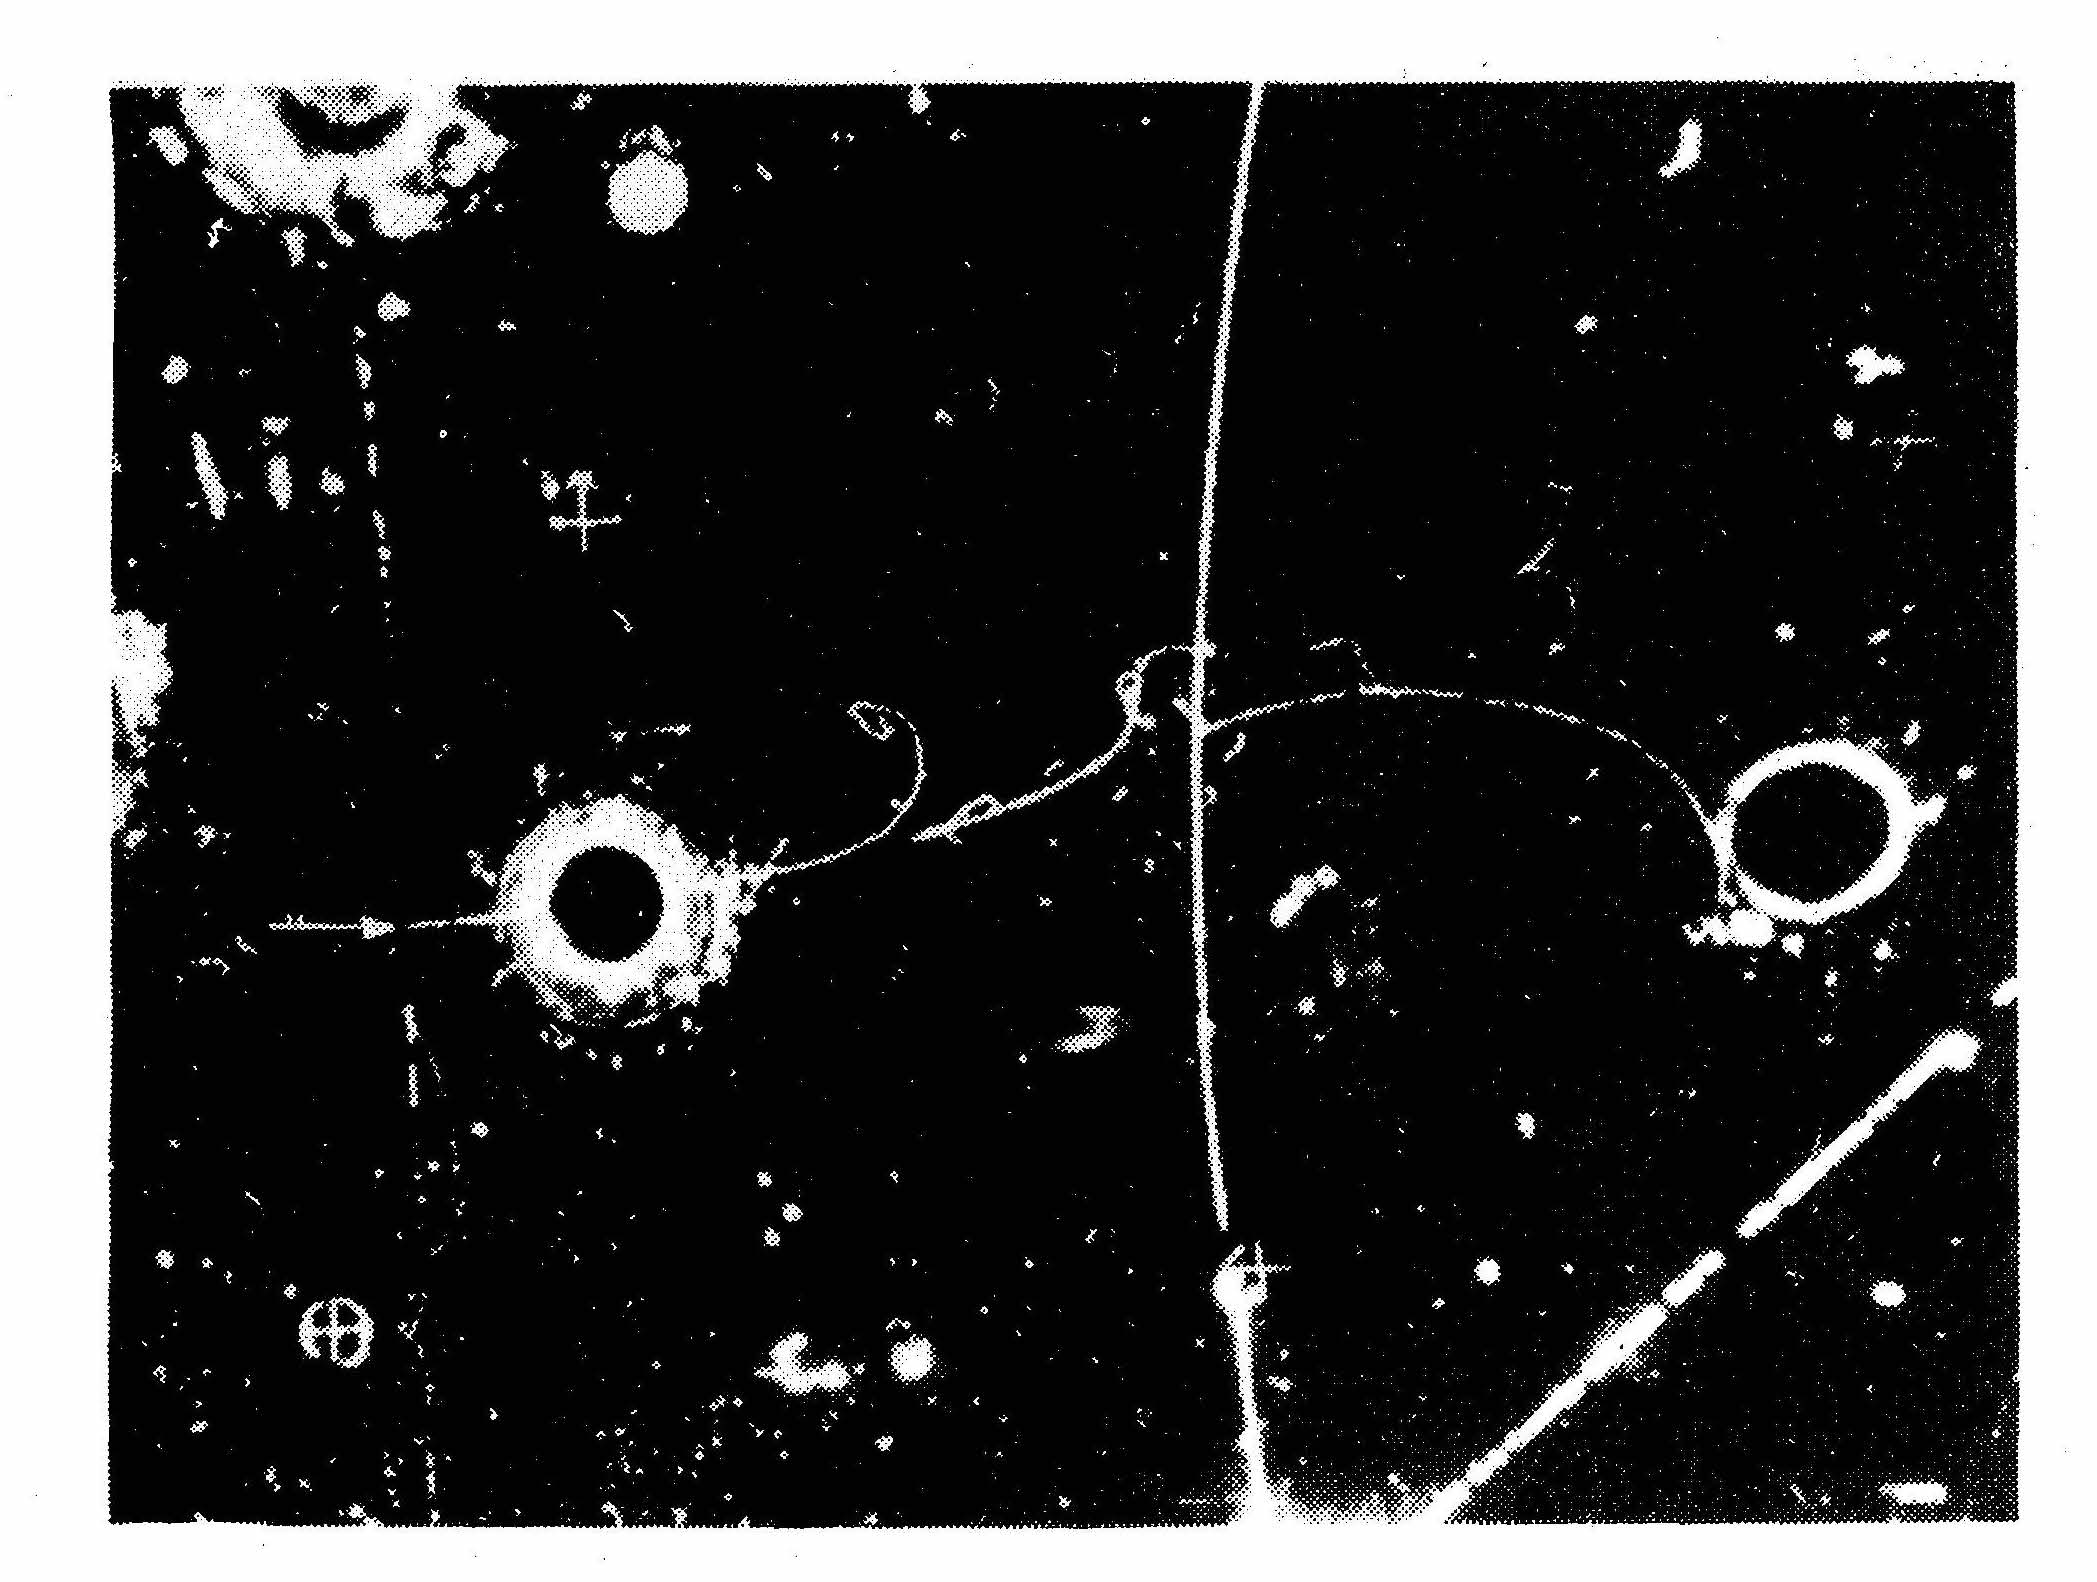
\includegraphics[width=0.45\textwidth]{images/Aachen.jpg}}


\begin{document}

\maketitle

\begin{frame}{Übersicht}
	\begin{Large}
  	\tableofcontents
	\end{Large}
\end{frame}

\section{Theoretical Introduction}
%\subsection{Parity}
\begin{frame}{Parity}
	The parity $\hat{P}$ operator transforms a phenomen into its mirror image.\\
	\begin{columns}
		\column{0.5\textwidth}
		$\hat{P} : \begin{pmatrix}
		t\\
		x\\
		y\\
		z\\
		\end{pmatrix} \mapsto \begin{pmatrix}
		t\\
		-x\\
		-y\\
		-z\\
		\end{pmatrix}$
		\column{0.5\textwidth}
		\begin{figure}
			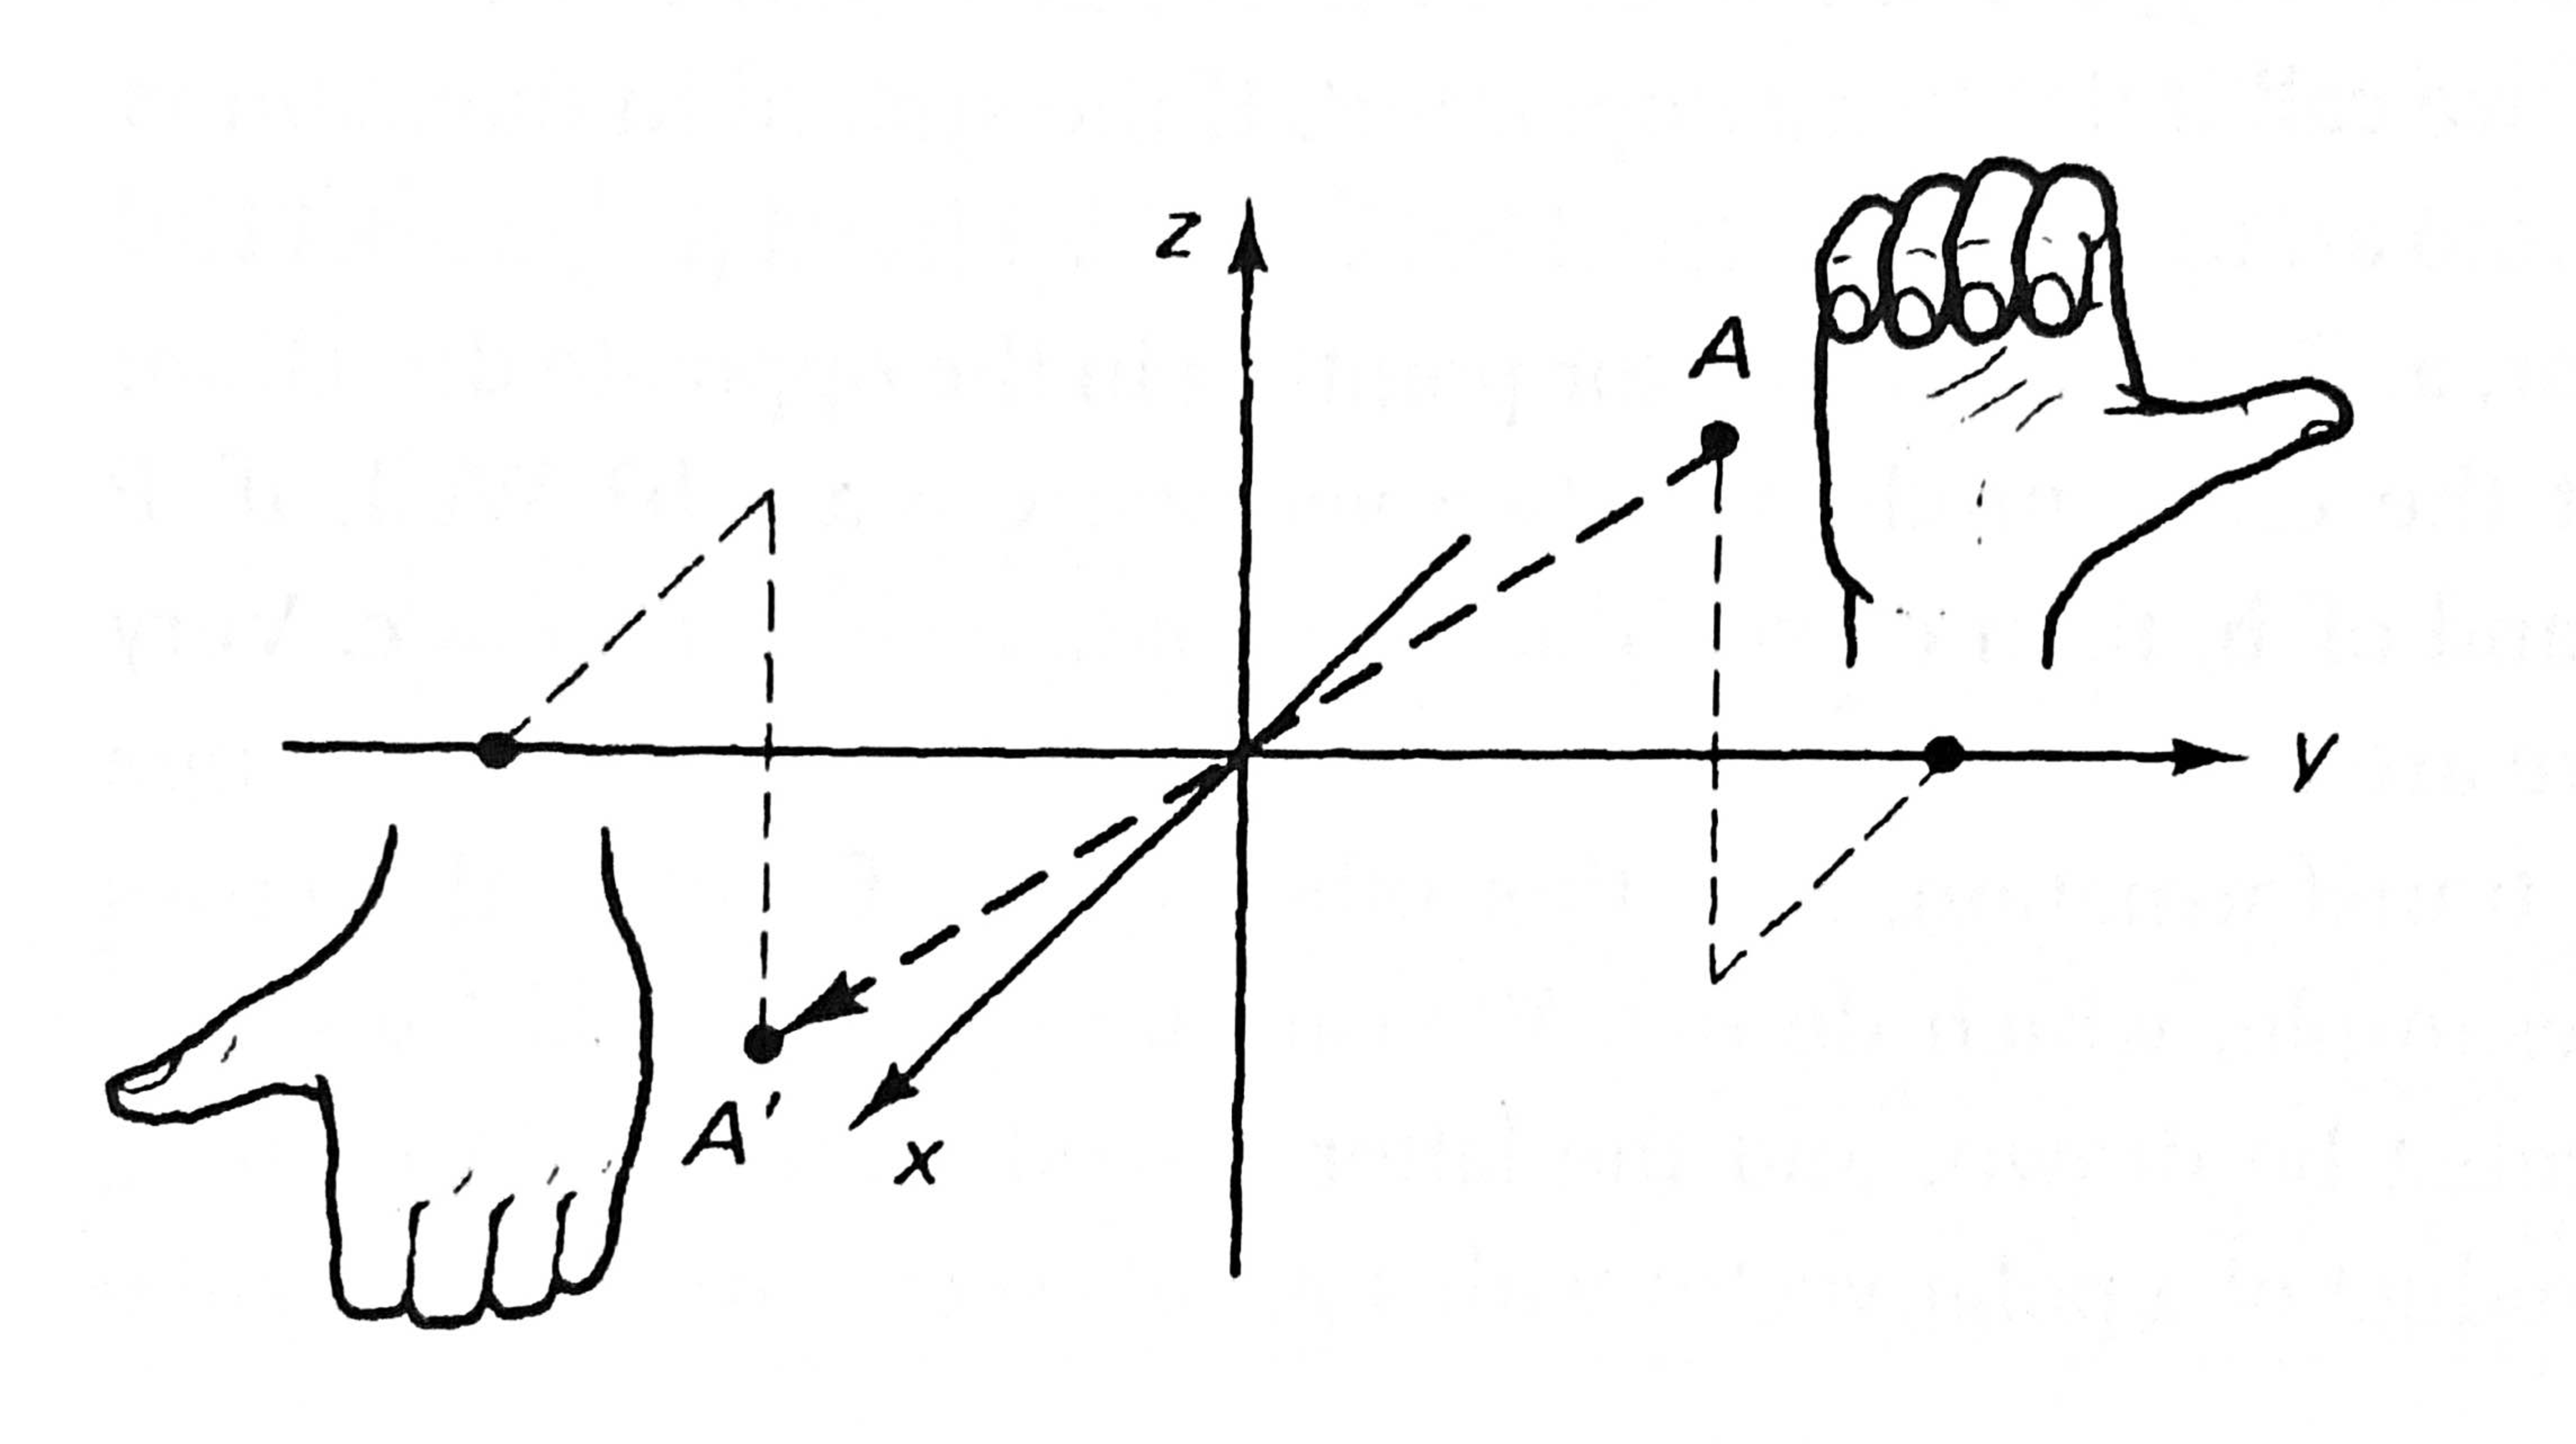
\includegraphics[width=0.55\textwidth]{images/parity_hand.pdf}
		\end{figure}
		\nocite{griffiths}
	\end{columns}
	Applying the parity operator two time transform a system in its original state.\\
	$\hat{P}^2=1$ \textrightarrow the eigen values are $\pm 1$.\\
	\underline{\textbf{Understanding of the SM in 1956}}
	\begin{itemize}
		\item the mirror image of any physical process shows the same physics \textrightarrow parity conservation \cite{feynman}
		\item a system is invariant under the combination of parity $\hat{p}$, charge conjugation $\hat{C}$ and time reversal $\hat{T}$\\
		\textrightarrow this is calles $CPT$~ theorem\\
		\textrightarrow assumption: each operation individually leaves the physics invariant as well\\
		\item former experiments showed that the electromagnetic and strong interaction conserves parity\\
		\textrightarrow assumption: same applies for the weak interaction
	\end{itemize}
\end{frame}

%\subsection{Reminder: Helicity and Chirality}
\begin{frame}{Reminder: Helicity and Chirality}
	Two imporant quantities to describe a particles movement:
	\begin{itemize}
		\item the direction of its momentum
		\item the particle spin $\vec{s}$
	\end{itemize}
	these can be described together:
	\begin{itemize}
		\item \textbf{helicity}: projection of the spin on the particle direction of movement\\
		\textrightarrow with two different possiblities
		\begin{enumerate}
			\item \underline{left-handed}: spin and the direction of movement are antiparallel
			\item \underline{right-handed}: spin and the direction of movement are parallel
		\end{enumerate}
		\item \textbf{chirality}: disassembly of a dirac spinor in two orthogonal states that transform under parity operation into each other
	\end{itemize}
	\begin{block}{value of chirality}
		\begin{itemize}
			\item a massless particle is lorentz-invariant \textrightarrow helicity $=$ chirality
			\item a chiral phenomenon is one that is not identical to its mirror image
		\end{itemize}
	\end{block}
\end{frame}

\begin{frame}{The $\tau$-$\theta$-puzzle}
	two charged strange Meson decays were observed:\\
	\vspace{0.2cm}
	\begin{columns}
		\column{0.3\textwidth}
		\begin{align*}
			\theta^+ &\rightarrow \pi^+ \pi^0\\
			\tau^+ &\rightarrow \pi^+ \pi^+ \pi^-
		\end{align*}
		\column{0.3\textwidth}
		\begin{align*}
			\hat{P}\ket{\theta} &= +1\ket{\theta}\\
			\hat{P}\ket{\tau} &= -1\ket{\tau}\\
		\end{align*}
		\column{0.4\textwidth}
	\end{columns}
	\vspace{0.2cm}
	\textrightarrow under the idea of parity conservation: two different particles\\
	\vspace{0.5cm}
	\textbf{problem}: same spin, charge, mass and lifetime\\
	adressed in 1953 by R.H. Dalitz as the $\tau$-$\theta$-puzzle \cite{doi:10.1080/14786441008520365}
\end{frame}

\begin{frame}{Is parity conserved in weak interactions?}
	Lee and Yang pointed out that the $\tau$-$\theta$-puzzle could describe the \textbf{same} particle. \cite{PhysRev.104.254}\\
	\textrightarrow this leads to the assumption that the weak interaction violates parity conservation\\
	\vspace{0.2cm}
	\underline{in case of parity nonconservation:}\\
	\begin{itemize}
		\item experimental states are mixture of usual and opposite parity ones
		\item the degree of mixing can be described by the fraction weight $\mathcal{F}^2$
		\item mixture would effect angular distributions of nuclear interactions
	\end{itemize}
	needs $\mathcal{F}^2$ to be small since selection rules worked, etc. \\
	\textrightarrow so far no experimental prove for parity conservation in weak interactions\\
	\vspace{0.2cm}
	\underline{numerous possiblities to do so:}
	\begin{itemize}
		\item angular distribution of $\beta$-decay between electron and nucleus
		\item $\beta-\gamma$-decays: polarization state of $\gamma$ to the electron
		\item meson decays: e.g. strange Meson with non vanishing spin
		\item angular distribution for $\pi-\mu-e$ decay
	\end{itemize}
\end{frame}

\begin{frame}{Angular distribution studies}
	framework uses two sets of operartors, parity conserving and nonconserving ones, leads to:
	\begin{itemize}
		\item $C$ coupling constant of parity conserving interaction
		\item $C^{'}$ coupling constant of parity nonconserving interaction
		\item $CC^{'}$ interference terms
	\end{itemize}
	previous measurements of $\beta$-decay quantities:\\
	\textrightarrow didn't contain interference terms $+$ $\nu$ spin needs to be measured to distinguish between $C$ and $C^{'}$\\
	\vspace{0.2cm}
	\underline{angular distribution:}\\
	$I(\vartheta) \text{d}\vartheta \propto (1 + \alpha \cos\vartheta)\sin\vartheta \text{d}\vartheta$\\
	with $\alpha$ asymmetry coefficient (contains interference terms $CC^{'}$)\\
	\vspace{0.2cm}
	\begin{columns}
		\column{0.5\textwidth}
		1) $\vartheta$ measured between oriented nuclei and emitted electron
		\begin{figure}
			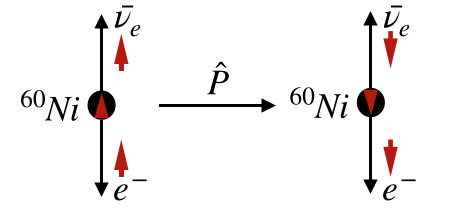
\includegraphics[width=0.4\textwidth]{images/parity_solinoid.png}
		\end{figure}
		\column{0.5\textwidth}
		2) $\vartheta$ measured between muon at rest and emitted electron\\
		$	\pi \rightarrow \mu + \nu$\\
			$\mu \rightarrow e + \nu + \nu$\\
		compare distributions for $\vartheta$ and $\pi - \vartheta$
	\end{columns}
\end{frame}

\section{The Wu Experiment}
\begin{frame}
	\begin{center}
		\begin{Large}
			The Wu Experiment\\
			angular destribtion study for nucleus $\beta$-decay
		\end{Large}
	\end{center}
\end{frame}

\begin{frame}{Principle of the Wu experiment}
	carried out at the National Bureau of Standards (NBS) in Washington, D.C.
	\begin{columns}[c]
		\column{0.5\textwidth}
		\begin{figure}
			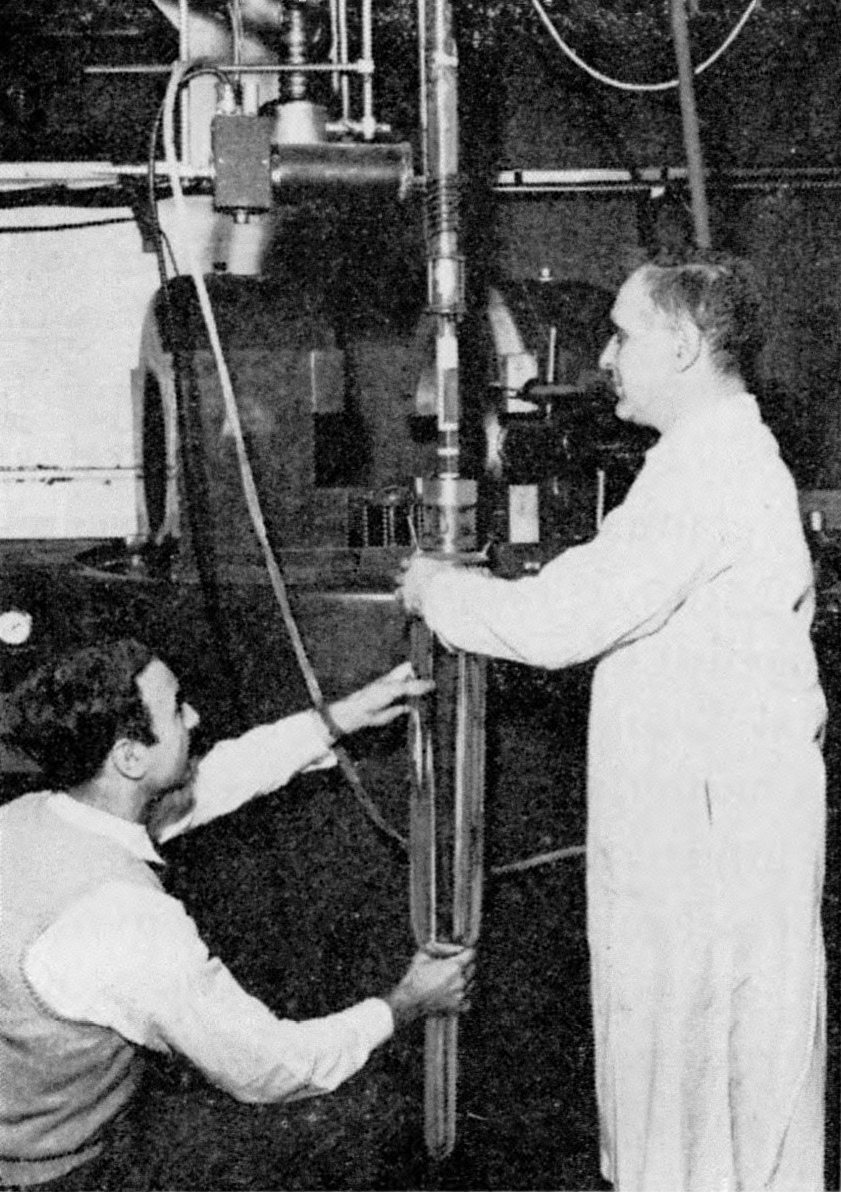
\includegraphics[width=0.55\textwidth]{images/Wu_experiment_NBS.jpg}
			\caption{Picture of the experimental setup of the Wu experiment.\cite{WuExperiment}}
			\label{fig:Wu1}
		\end{figure}
		\column{0.5\textwidth}
		\underline{Principle of the measurement}\nocite{PhysRev.105.1413}
		\begin{itemize}
			\item $\beta$-decay of a nucleus to verify if the weak interaction is chiral or not
			\item changing the direction of polarization of the nuclei is equivalent to a parity operation
			\item measure the angular distribution of the electrons\\
			\textrightarrow check if independent from the nucleus polarization
		\end{itemize}
		\begin{figure}
			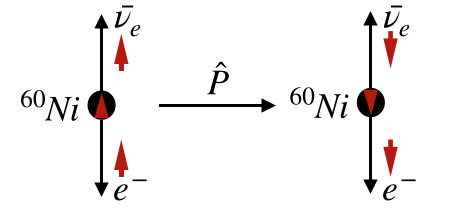
\includegraphics[width=0.7\textwidth]{images/parity_solinoid.png}
			%\caption{Picture of C.-S. Wu, Y.K. Lee, and L.W. Mo.\cite{WuBild}}
			\label{fig:Wu3}
		\end{figure}
	\end{columns}
\end{frame}

% \begin{figure}
% 	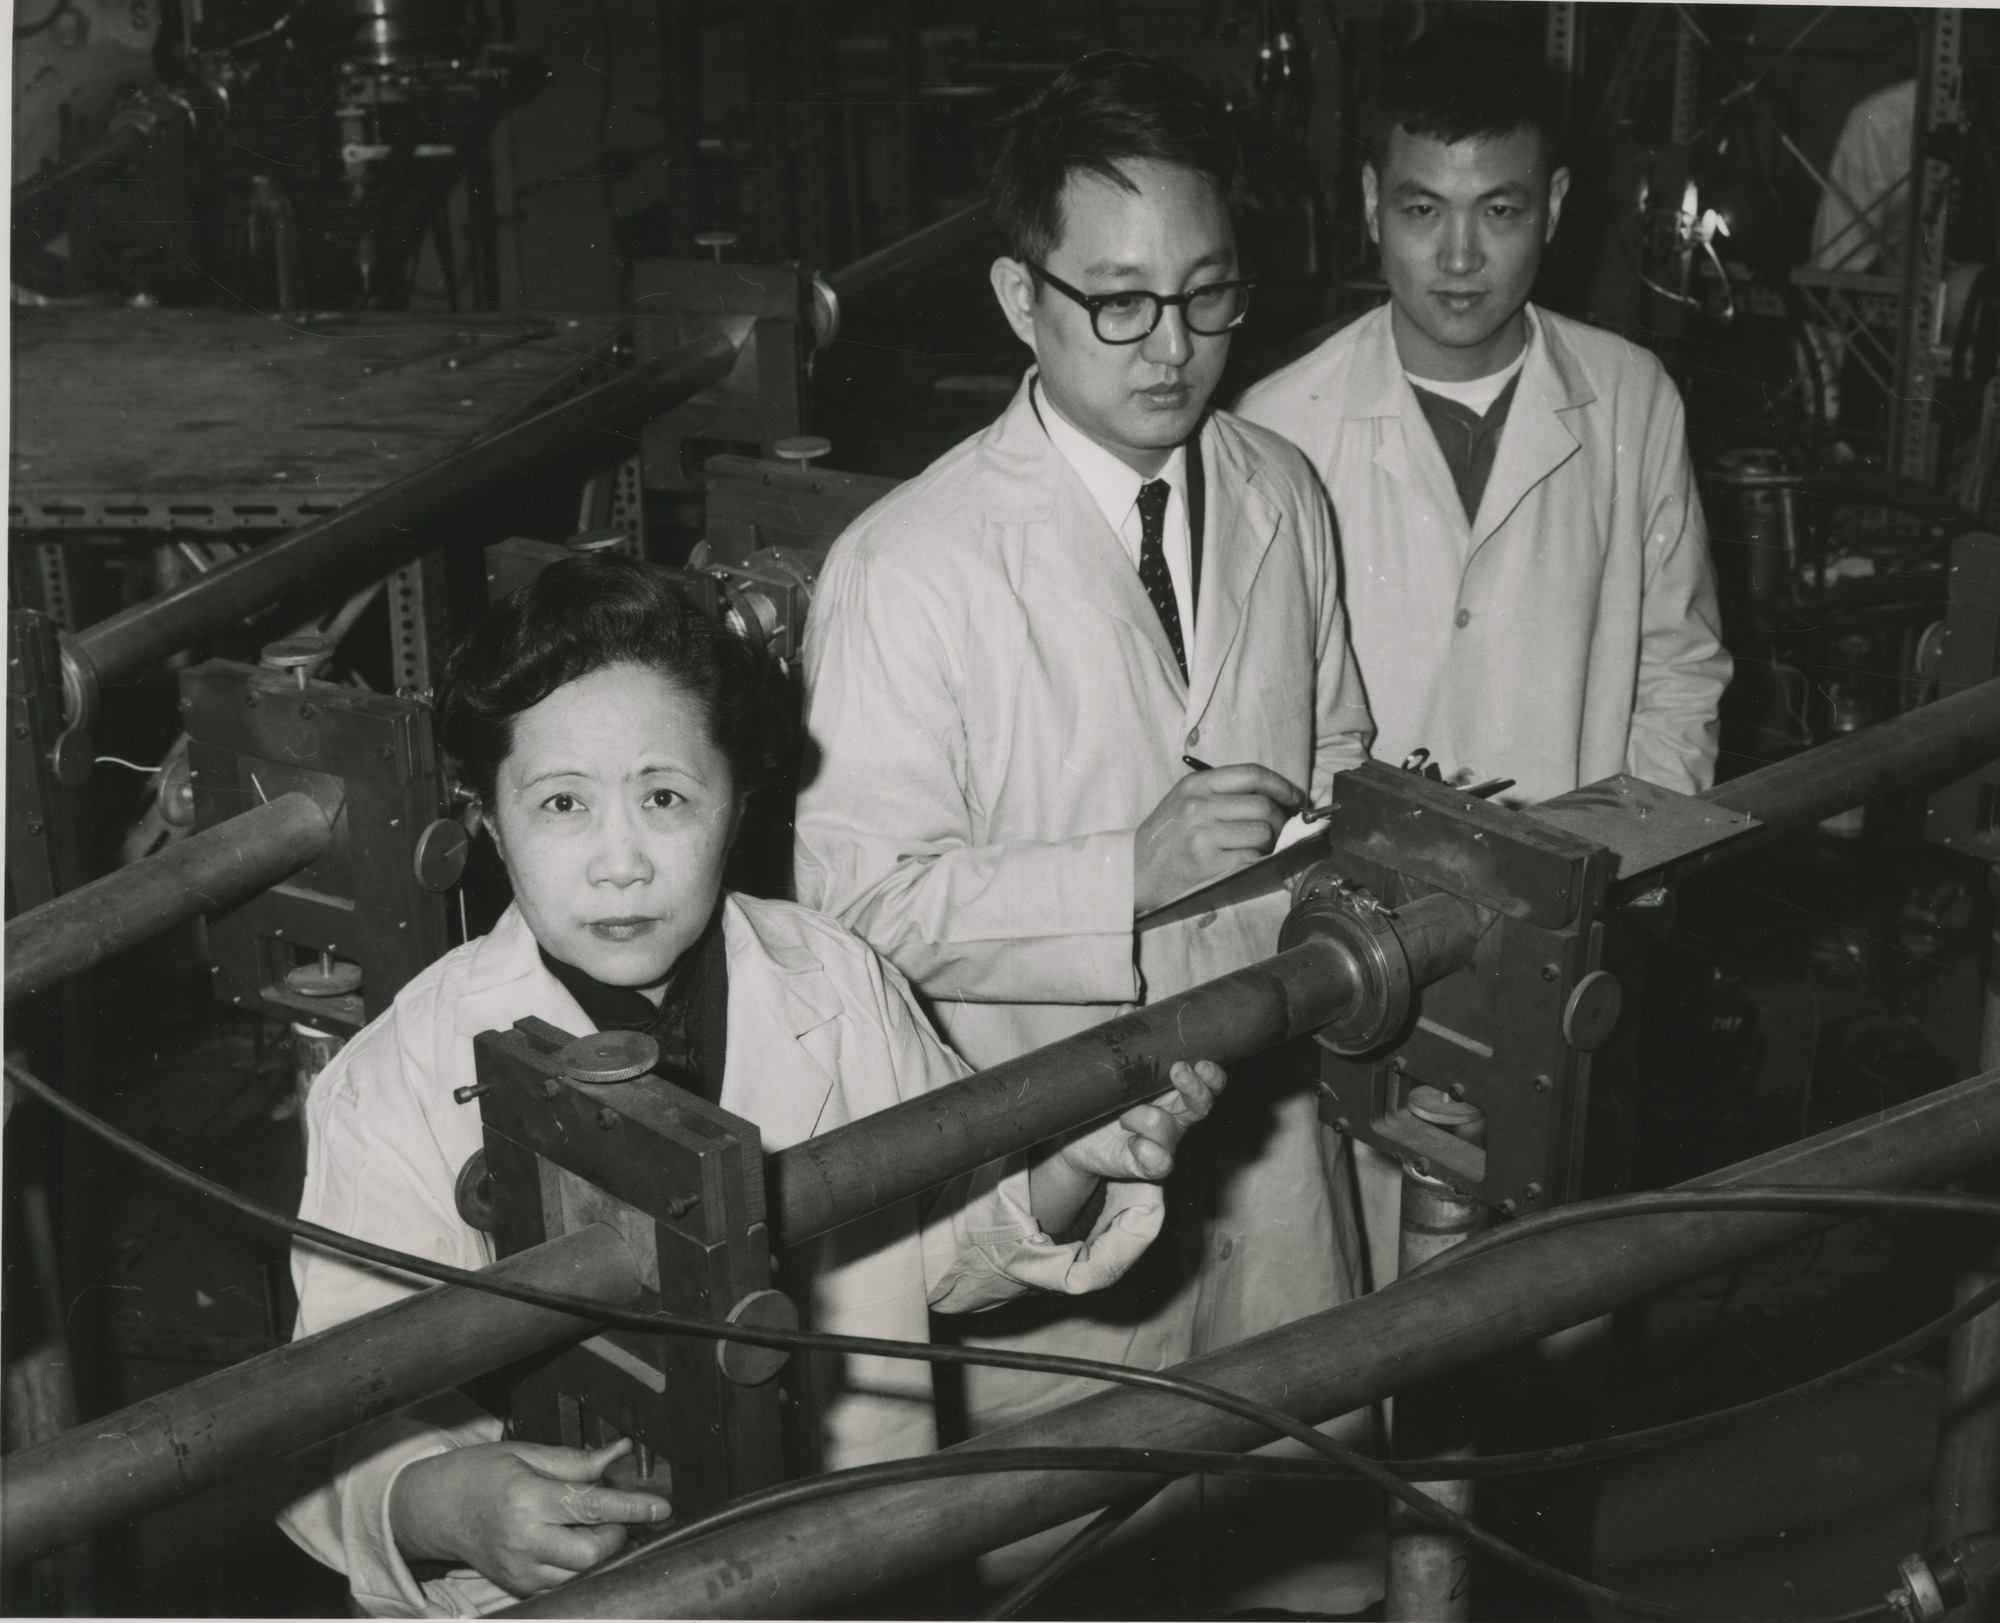
\includegraphics[width=0.4\textwidth]{images/Wu_Lee_Mo.jpg}
% 	\caption{Picture of C.-S. Wu, Y.K. Lee, and L.W. Mo.\cite{WuBild}}
% 	\label{fig:Wu2}
% \end{figure}

\begin{frame}{The experimental setup}
	\begin{columns}
		\column{0.5\textwidth}
		\begin{figure}
			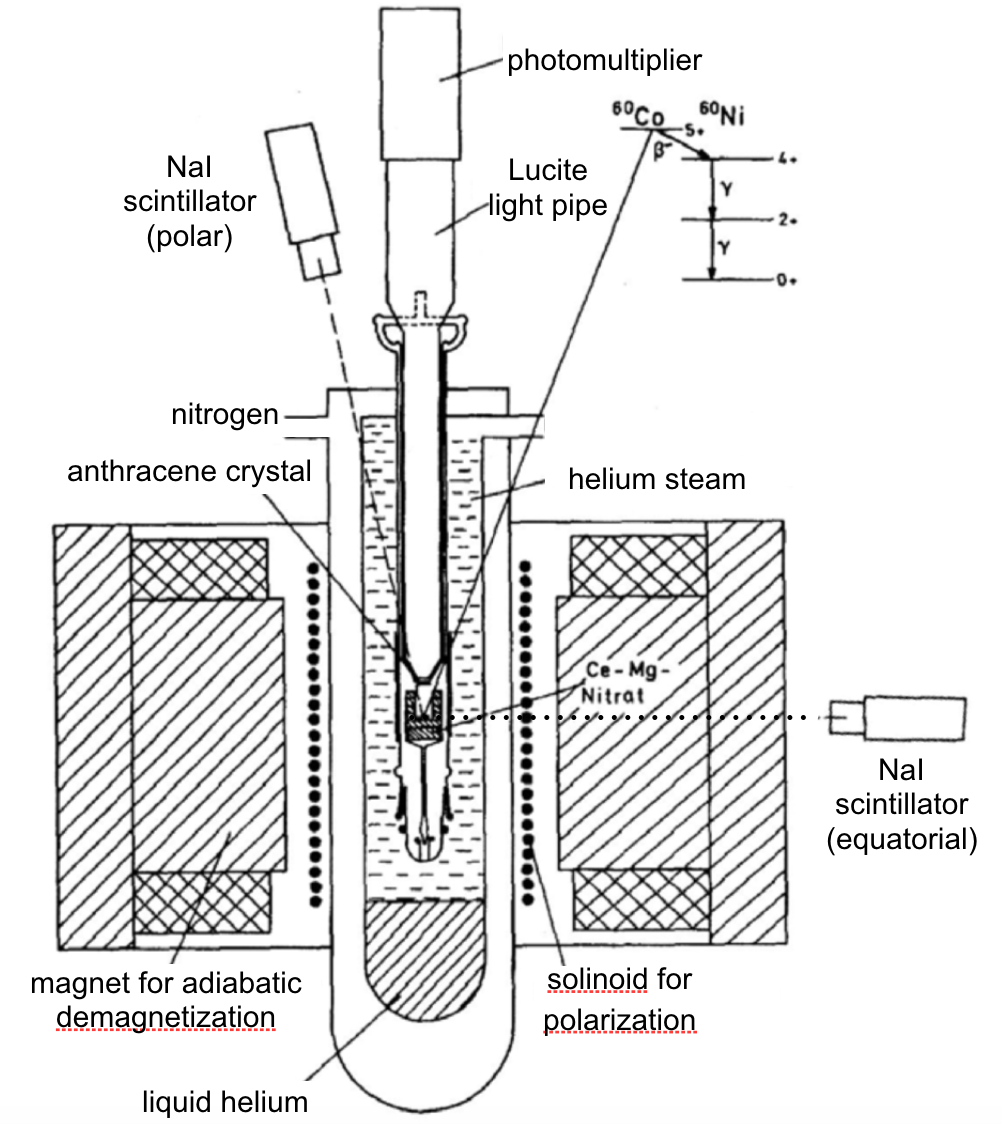
\includegraphics[width=0.82\textwidth]{images/Wu_setup.png}
		\end{figure}
		\nocite{wegener}
		\column{0.5\textwidth}
		\underline{Setup components}
		\begin{itemize}
			\item anthracen crystall \textrightarrow $\beta$ particle detection
			\item Lucite light pipe with photomultiplier
			\item two NaI gamma scintillator
			\item specimen: cerium magnesium nitrate crystal with vaporised layer of $^{60}Co$
			\item cooling system \textrightarrow helium (nitrogen), magnet (adiabatic demagnetization)
			\item solinoid \textrightarrow polarization
		\end{itemize}
		\underline{difficulties}
		\begin{itemize}
			\item anthracen crystal needs to be inside of the cryostat
			\item polarization of the nuclei
		\end{itemize}
	\end{columns}
\end{frame}

\begin{frame}{Selection of the right nucleus}
	\begin{columns}
		\column{0.5\textwidth}
		There are two types of $\beta$ decay
		\begin{itemize}
			\item \textbf{Fermi transition}: particles have antiparallel spin ($\Delta  S = 0$)
			\item \textbf{Gamow-Teller transition}: particles have parallel spin ($\Delta S = 1$)
		\end{itemize}
		\textrightarrow if weak interaction is chiral only a Gamow-Teller transition\\
		 can prove that\\
		\textrightarrow $^{60}Co$ has a Gamow-Teller $\beta$ decay\\
		\begin{align*}
			^{60}Co &\rightarrow ^{60}Ni + e^- + \bar{\nu_{e}} + 2\gamma\\
			I_{z,Co} &= I_{z,Ni} + I_{z,e} + I_{z,\nu} = 5 \\
			I_{z,Ni} &= 4\\
			I_{z,e} &= I_{z,\nu} = \frac{1}{2}
		\end{align*}
		\column{0.5\textwidth}
		\begin{figure}
			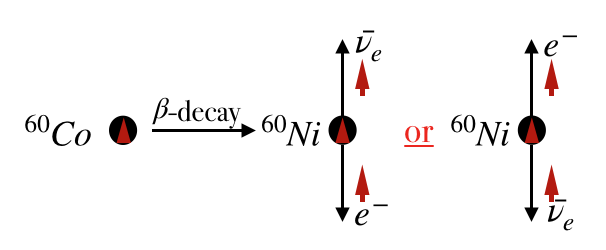
\includegraphics[width=0.85\textwidth]{images/Co_beta.png}
		\end{figure}
		\underline{Second benefit}
		\begin{itemize}
			\item photons are emitted in the direction of the nucleus polarization\\
			\textrightarrow indicator of polarization degree
			\item controll of the polarization of the emitted electrons
		\end{itemize}
	\end{columns}
\end{frame}

\begin{frame}{Polarization of nuclei}
	nuclear moments can couple to an external field \textrightarrow aligns nuclear spin\\
	\vspace{0.2cm}
	\textbf{\textrightarrow problem}: surrounded by electrons $\mu_{N} \ll \mu_{B}$\\
	\vspace{0.2cm}
	\underline{nuclear Polarization factor} according to M. E. Rose \cite{PhysRev.75.213}:\\
	\begin{columns}
		\column{0.4\textwidth}
		\begin{align*}
			f_{N} = \frac{1}{I}\frac{\sum m_{i}\exp{-\frac{m_{i}\mu_{N}H}{k_{B}TI}}}{\sum\exp{-\frac{m_{i}\mu_{N}H}{k_{B}TI}}}\\
			\Longrightarrow f_{N}\left(\frac{m_{Ni}=4}{m_{Co}=5}\right) \propto \exp{-\frac{g \mu_{N}B}{k_{B}T}}
		\end{align*}
		\column{0.1\textwidth}
		\column{0.4\textwidth}
		\underline{requirements for the polarization}
		\begin{itemize}
			\item strong magnetic field
			\item temperature close to absolute zero
		\end{itemize}
	\end{columns}
	\vspace{0.5cm}
	at $T=\SI{1}{\kelvin}$ and $B=\SI{1}{\tesla}$ is $\mu_{N} \propto \mathcal{O}\left(\frac{\mu_{B}}{1000}\right)$\\
	\vspace{0.2cm}
	\textrightarrow just enough to polarise the shell electrons, not the nucleus
\end{frame}

\begin{frame}{Gorter-Rose method for nucleus polarization}
	\begin{itemize}
		\item 1948: Gorter \cite{GORTER1948504} and Rose \cite{PhysRev.75.213} describe the possiblity of polarising a nucleus by adiabatic demagnetization\\
		\underline{process}:\\
		\begin{columns}
			\column{0.4\textwidth}
				\begin{figure}
					\center
					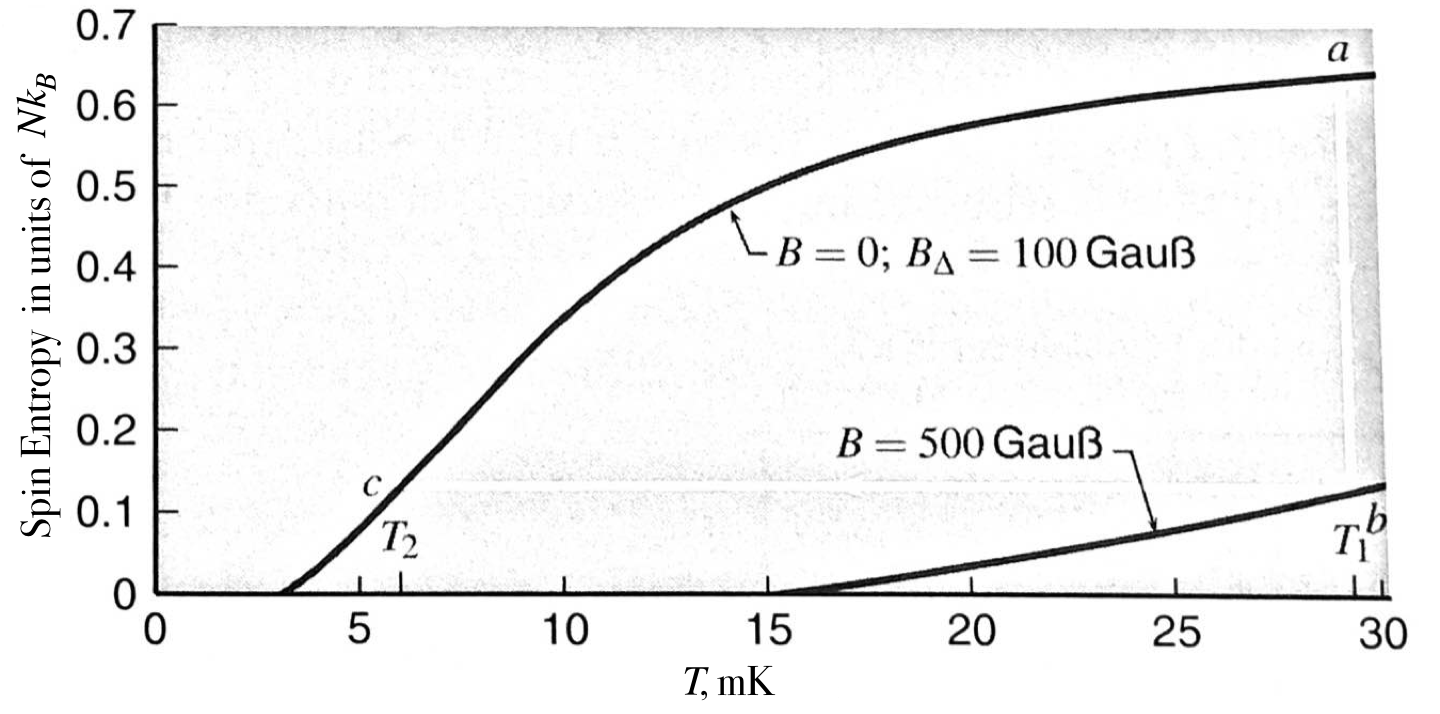
\includegraphics[width=0.9\textwidth]{images/adiabatic_demag.png}
					\caption{Principle of adiabatic demagnetization.\cite{kittel}}
				\end{figure}
			\column{0.6\textwidth}
			\begin{enumerate}
				\item magnetic field reduses the entropy of the magnetic moments in the salt ($B_{1} \sim \SI{1}{\tesla}$)
				\item adiabatic isolation and switching off the magnetic field
				\item entropy corresponds to a lower temperature \textrightarrow cooling to $\sim \SI{0.003}{\kelvin}$
			\end{enumerate}
		\end{columns}
		\item small magnetic field $B_{2}$ vertical to cooling magnet (here solinoid)\\
		\textrightarrow polarization of the shell electrons causes $\sim \SI{1}{\tesla}$ field \textrightarrow polaises the nucleus
		\item using CeMg nitrate with a high anisotropic Landé g-factor ($g_{1} \ll g_{2}$)
		\item 1953: method successfully tested for $^{60}Co$ \cite{doi:10.1080/14786440208520296}
	\end{itemize}
\end{frame}


\begin{frame}{Results of the experiment}
	\textrightarrow $\SI{60}{\percent}$ of the nuclei are polarised \nocite{PhysRev.105.1413}\nocite{WuExperiment}
	\begin{columns}
		\column{0.3\textwidth}
		\begin{figure}
			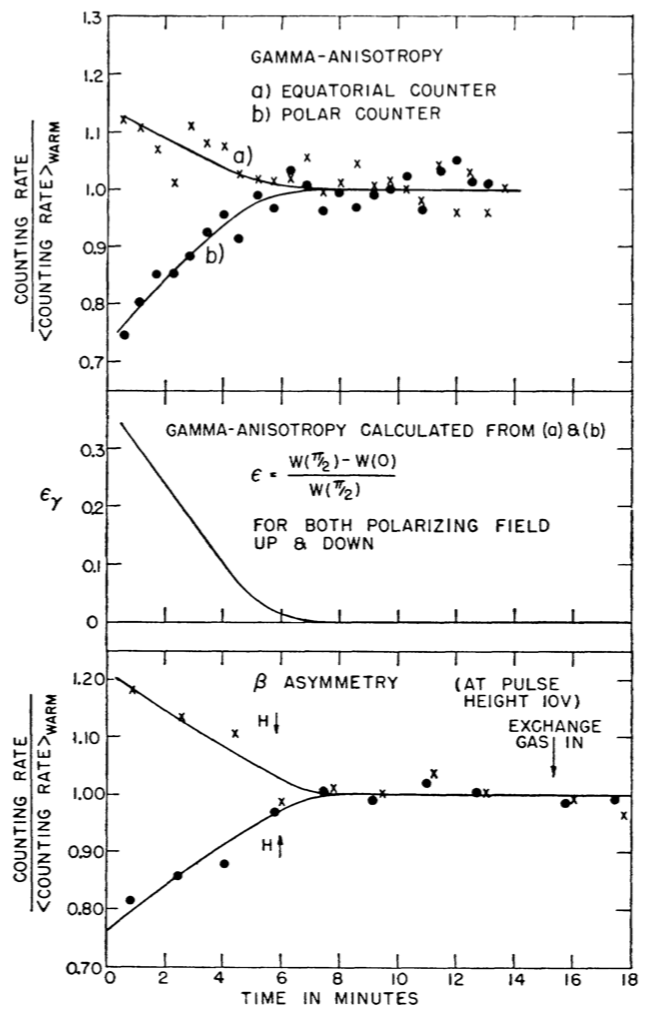
\includegraphics[width=0.9\textwidth]{images/Wu_result.png}
		\end{figure}
		\column{0.4\textwidth}
		\begin{figure}
			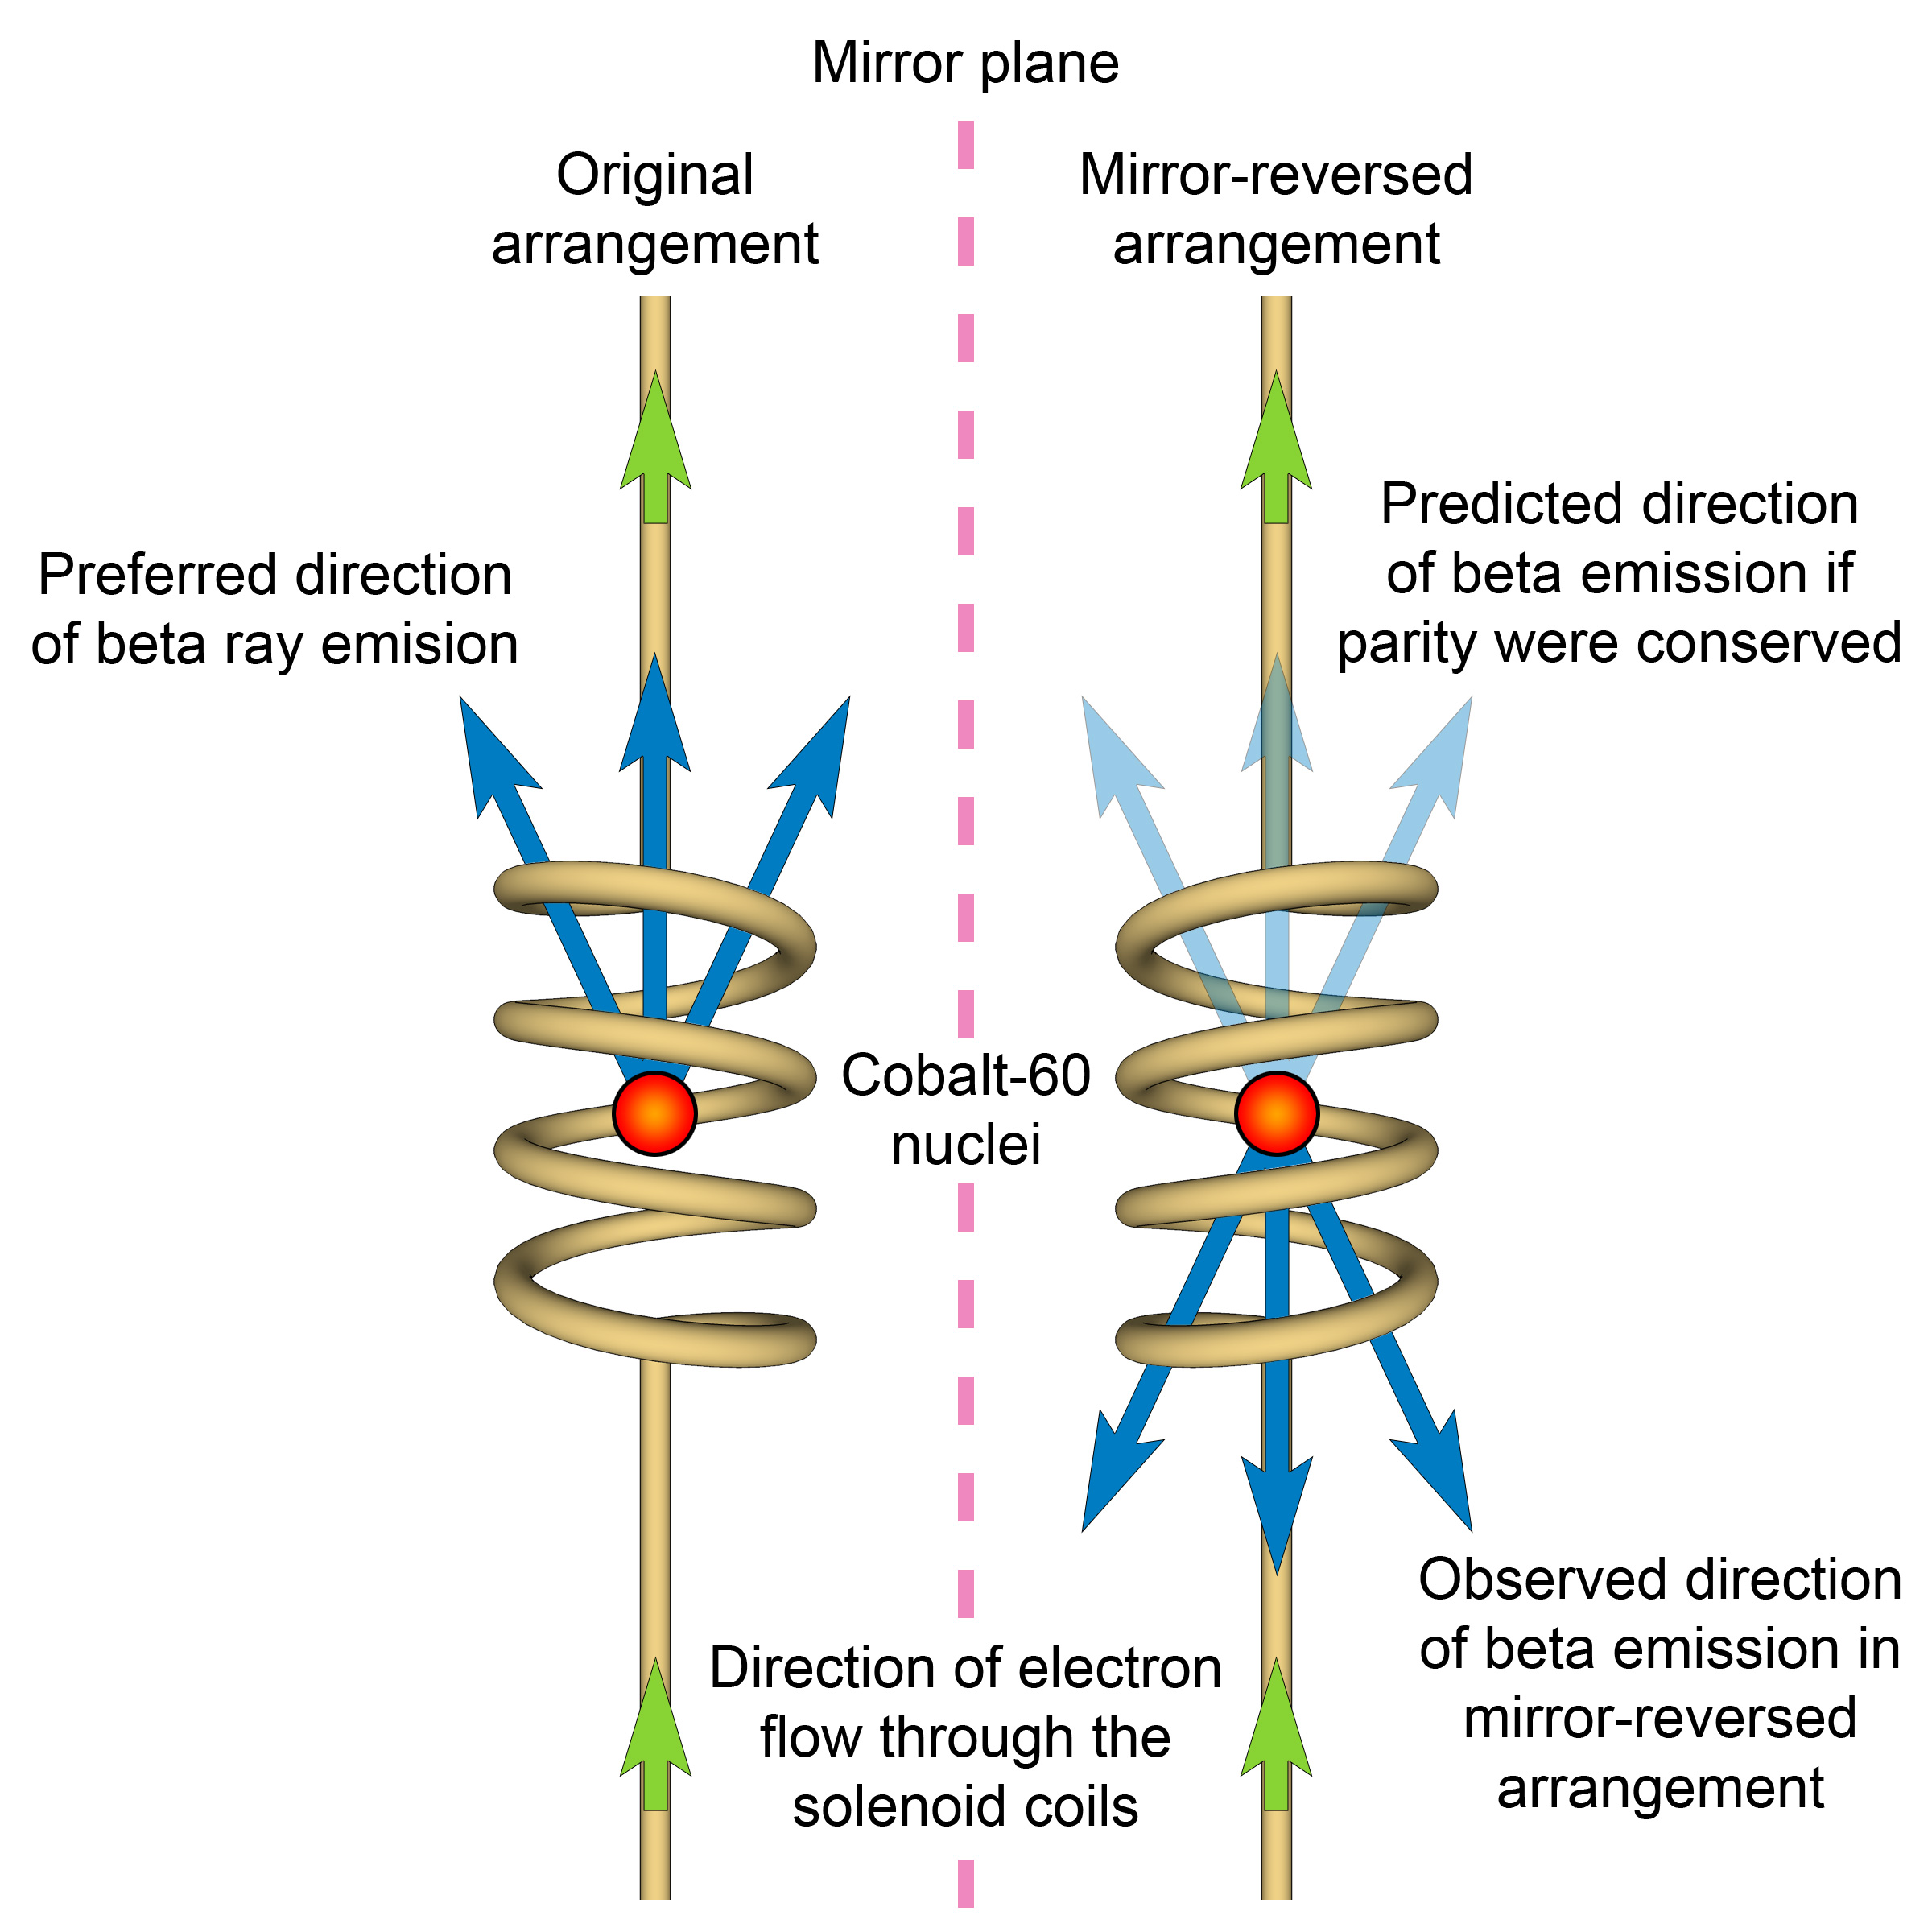
\includegraphics[width=\textwidth]{images/Wu_experiment.jpg}
		\end{figure}
		\column{0.3\textwidth}
		\underline{observation}
		\begin{figure}
			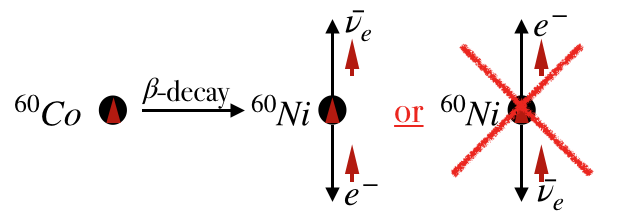
\includegraphics[width=0.8\textwidth]{images/Co_violation.png}
		\end{figure}
		\begin{itemize}
			\item asymmetry in the observed angular distribution of the electron for $\theta$ and $180^° -\theta$
			\item the observed $\beta$ asymmetry matches exactly the observed gamma anisotropy
		\end{itemize}
	\end{columns}
\end{frame}

\begin{frame}{Results and cross checks}
	\underline{reminder}\\
	\vspace{0.2cm}
	$I(\vartheta) \text{d}\vartheta \propto (1 + \alpha \cos\vartheta)\sin\vartheta \text{d}\vartheta$\\
	with $\alpha$ asymmetry coefficient (contains interference terms $CC^{'}$)\\
	\begin{columns}
		\column{0.6\textwidth}
		\begin{block}{result}
			$\alpha \sim -0.4$ for a velocity of $\frac{v}{c}\approx 0.6$\\
			\textrightarrow $\beta$ particle more favoured in opposite direction of nucleus spin
		\end{block}
		\column{0.4\textwidth}
	\end{columns}
	\vspace{0.2cm}
	\underline{cross checks}
	\begin{enumerate}
		\item check for remanent magnetization by reversal of the direction of the demagnetization field \textrightarrow no effect
		\item check if a small magnetic field can cause the asymmetry (misalignment)\textrightarrow $CoCL_{2}$ solution on the bottom of the housing \textrightarrow disturbs cooling \textrightarrow no $\beta$ asymmetry was seen
		\item check if internal magnetic effects change the electron path to the surface \textrightarrow dissolve the crystal surface with the $CoCL_{2}$ solution \textrightarrow no $\beta$ asymmetry was seen
	\end{enumerate}
\end{frame}

\begin{frame}{Interpretation by Lee and Yang}
	The observed asymmetry in the angular distributions shows a maximum violation of parity conservation. \\
	\textrightarrow the weak interaction is chiral\\
	\begin{block}{quote from the paper\cite{PhysRev.105.1413}}
		"According to Lee and Yang\cite{PhysRev.106.340} the present experiment indicates\\ not only that conversation of parity is violated but also\\ that invariance under charge conjugation is violated."
	\end{block}
	\vspace{0.2cm}
	This was a false conclusion!\\
	By the time it was believed that $CP$ is also conserved, so if parity conservation is violated\\
	\textrightarrow invariance under charge conjugation as well
\end{frame}

\section{The Columbia experiment}

\begin{frame}
	\begin{center}
		\begin{Large}
			The Columbia Experiment\\
			angular destribtion study for $\pi^{+}-\mu^{+}-e^{+}$-decay
		\end{Large}
	\end{center}
\end{frame}

\begin{frame}{The Columbia experiment}
	After Lee and Yang reported that the Wu experiment proved parity violation in a conversation\\
	L.M. Lederman, R.L. Garwin and his gradute student M. Weinrich examine the $\pi-\mu-e$ angular distribution \cite{PhysRev.105.1415}\\
	\vspace{0.2cm}
	\underline{concept:}\\
	if parity conservation is violated the muons are highly polarised:
	\begin{figure}
		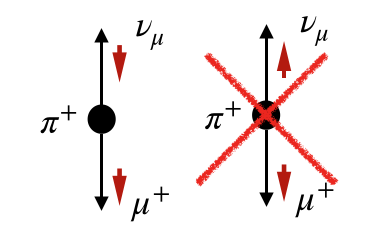
\includegraphics[width=0.25\textwidth]{images/muon_polarization.png}
	\end{figure}
	\vspace{0.2cm}
	electron spin is the same as the muon spin (conversation of momentum)\\
	in this case they should measure asymmetric angular distributions for $\vartheta$ and $\pi - \vartheta$\\
\end{frame}

\begin{frame}{The experimental setup}
	\begin{columns}
		\column{0.5\textwidth}
		\begin{figure}
			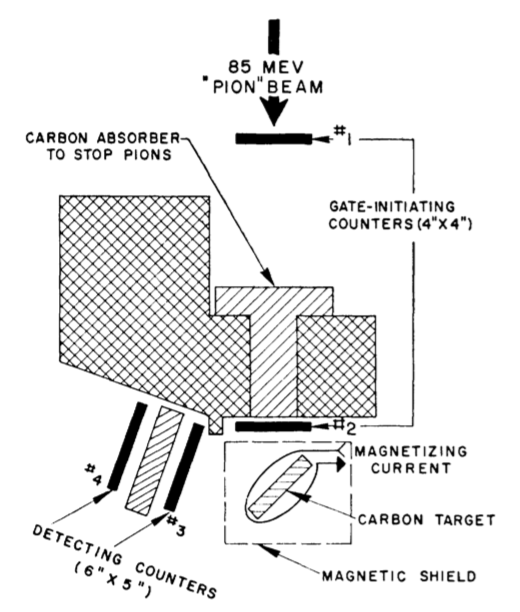
\includegraphics[width=0.75\textwidth]{images/muon_setup.png}
		\end{figure}
		\column{0.5\textwidth}
		\underline{Setup components}
		\begin{itemize}
			\item $\SI{85}{\mega\electronvolt}$ pion beam provided by a cyclotron
			\item $\SI{20}{\centi\meter}$ carbon target to stop the pions
			\item $\SI{2.5}{\centi\meter}$ carbon target to stop the muons
			\item fast coincidence between counter 1 and 2 \textrightarrow stopped muons
			\item electron telescope out of counter 3 and 4 ($E_{e} \rangle \SI{25}{\mega\electronvolt}$)
			\item delayed coincidence between 1+2 and 3+4 \textrightarrow just muon decay electrons
			\item rectangular solinoid above the muon carbon target
		\end{itemize}
	\end{columns}
\end{frame}

\begin{frame}{Results}
	\underline{reminder}\\
	\vspace{0.2cm}
	$I(\vartheta) \text{d}\vartheta \propto (1 + \alpha \cos\vartheta)\sin\vartheta \text{d}\vartheta$\\
	with $\alpha$ asymmetry coefficient (contains interference terms $CC^{'}$)\\
	$\vartheta$ is measured between the muon velocity vector and the electron, assumption that the gyromagnetic ratio is $+2.00$\\
	\begin{columns}
		\column{0.5\textwidth}
		\begin{figure}
			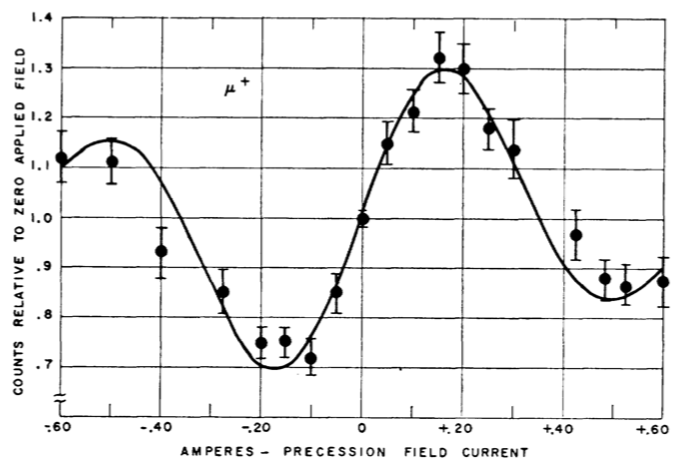
\includegraphics[width=0.6\textwidth]{images/result_muon.png}
		\end{figure}
		\column{0.5\textwidth}
		\begin{figure}
			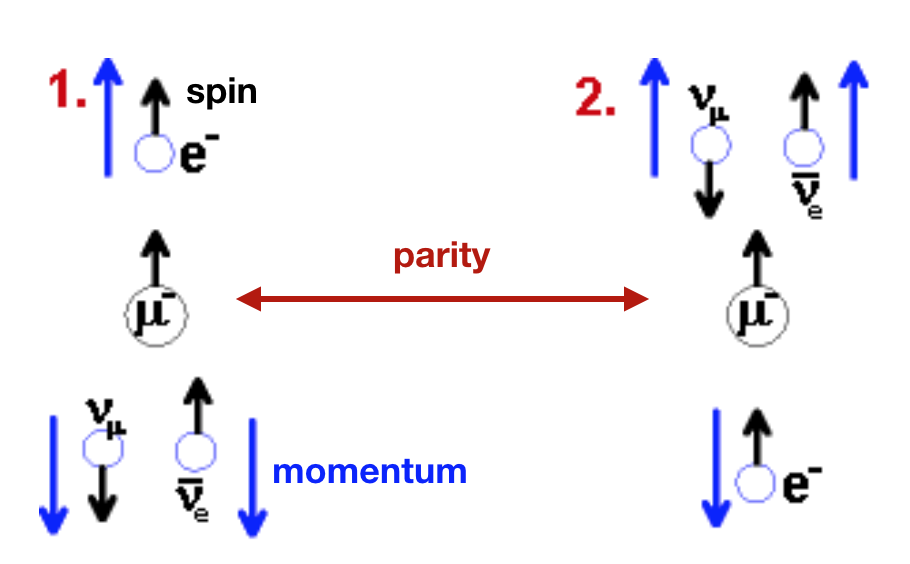
\includegraphics[width=0.6\textwidth]{images/muon_decay.png}
		\end{figure}
	\end{columns}
	\nocite{muon}
	\textbf{results}: \\
	large asymmetry was observed with $\alpha = -0.33 \pm 0.03$ from fit of $(1 + \alpha \cos\vartheta)$\\
	\textrightarrow shows again that parity and charge conservation is violated (same results where seen for $\mu^{-}$ decay)
\end{frame}

\section{Chronological Development}
\begin{frame}{Chronology of the discovery of parity violation}
	\startchronology[startyear=1925,stopyear=1935,height=0.5ex]
		\chronoevent[textwidth=6cm]{1928}{Cox \cite{Cox544} and Chase \cite{Chase} start studying double scattering of beta rays actuall first proof of parity violation}
		\chronoevent[textwidth=5cm]{1933}{Fermi and Pauli propose the $\beta$ decay}
	\stopchronology
	\startchronology[startyear=1955,stopyear=1958,height=0.5ex]
		\chronoevent[textwidth=5cm]{1956}{Yang gives a talk at a conference in April, Yang + Lee submit the paper of parity violation in June}
		\chronoevent[textwidth=5cm]{1957}{early: Wu+Lederman publish their results on parity violation, later Telegdi + Friedman\cite{PhysRev.105.1681.2}, late: Goldhaber experiment confirms that neutrinos are left-handed\\}
		\chronoevent[textwidth=4cm]{1958}{Sudarshan+Marshak/Feynman+Gell-Mann: develop V-A structure}
	\stopchronology
	\nocite{nobelprize}\nocite{Hadjiivanov:2018lgp}
\end{frame}


\section{Conclusion}

\begin{frame}{Conclusion}
	\begin{Large}
	 \begin{itemize}
	  	\item both experiments showed a high asymmetry in the angular distributions
	  	\item that shows that the electron and the muon are highly polarised
	  	\item prove that parity violation is maximal
	  	\item therefore the weak interaction must be chiral
	  	\item at this point it wasn't proved that neutrinos are left-handed\\ (later proved by the Goldhaber experiment)
		\end{itemize}
	\end{Large}
\end{frame}



\begin{frame}
  \begin{center}
    \begin{Large}
			Thank you for your attention.\\
			Questions? \nocite{wegener}
	  \end{Large}
  \end{center}
\end{frame}


\section*{Literatur}
\begin{frame}[allowframebreaks]{Literatur}
  \printbibliography
\end{frame}

\end{document}
